%%%%%%%%%%%%%%%%%%%%%%%%%%%%%%%%%%%%%%%%%%%
%%%%%%%%%%%%%%%%%%%%%%%%%%%%%%%%%%%%%%%%%%%
%%%%%%%%%%%%%%% CHAPTER 03 %%%%%%%%%%%%%%%%


\section{Transformada inversa de Laplace}

\frame{
\frametitle{Relembrando}
\begin{block}{Transformada de Laplace}
A transformada de Laplace foi definida no capítulo anterior como sendo:
$$\mathscr{L}\{f(t)\} \triangleq \int_{0}^{\infty} f(t) \ e^{-st} \text{d}t \triangleq F(s)$$
\end{block}
}

\frame{
\frametitle{Unicidade}
\begin{block}{A função é definida apenas para $t>0$}
Lembrando que uma das condições de existência da transformada de Laplace é que $f(t)$ seja igual a 0 para $t < 0$, sabemos então que a forma de $f(t)$ para os reais negativos não influencia a integração. \\
\begin{itemize}
    \item \textbf{Exemplo}: $F_1(s) = F_2(s) = F_3(s)$
\end{itemize}
\end{block}
\vspace{0.2cm}
\centerline{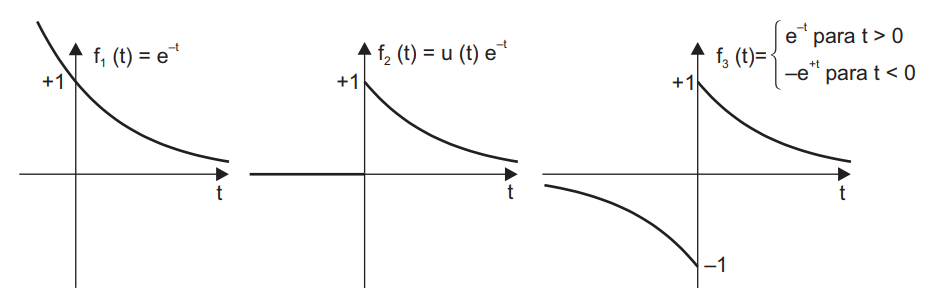
\includegraphics[width=1\linewidth]{Figuras/Ch03/fig1.PNG}}
}

\frame{
\frametitle{Inversão da transformada}
\begin{block}{Teorema da unicidade}
\begin{itemize}
    \item Com o objetivo de fazer existir uma única $f(t)$ para cada $F(s)$ é que impomos a condição de $f(t)$ ser zero para $t < 0$. Consequentemente, somente a função $f_2(t)$ é transformável.
    \item Quando é colocada a condição de $f(t) = 0$ para $t < 0$ para a \textbf{unicidade}, isto leva à existência de uma fórmula que nos permite, a partir de $F(s)$, determinar $f(t)$.
    \item O \textbf{teorema da unicidade} garante que, se $f(t)$ for \textbf{contínua}, para a função $f(t)$ há \textbf{uma e somente uma} 
    $F(s)$. Como $f(t)$ é igual a zero para $t < 0$, então uma dada $F(s)$ corresponde a somente uma $f(t)$.
\end{itemize}
\end{block}
}

\frame{
\frametitle{Inversão da transformada}
\begin{block}{Definição}
Se $F(s) = \mathscr{L}\{f(t)\}$ é a transformada de Laplace de $f(t)$, então dizemos que $f(t) = \mathscr{L}^{-1}\{F(s)\}$ é a \textbf{transformada inversa de Laplace} de $F(s)$.
\vspace{0.2cm}
\begin{itemize}
    \item Essa definição só faz sentido se a transformação definida no conjunto de funções que possuem transformada de Laplace for \textbf{bijetora}, ou seja, cada função $f(t)$ está relacionada a uma única transformada $F(s)$. 
\end{itemize}
\end{block}
}

\frame{
\frametitle{Propriedade}
\begin{block}{Superposição}
Considere uma função $F(s)$ cuja transformada inversa de Laplace é $f(t)$, e considere ainda uma função $G(s)$ cuja cuja transformada inversa de Laplace é $g(t)$. Deste modo:

$$\mathscr{L}^{-1}\{\alpha F(s) + \beta G(s)\} = \alpha f(t) + \beta g(t)$$ \\
\vspace{0.2cm}
\textbf{Demonstração}: 
$$\mathscr{L}^{-1}\{\alpha F(s) + \beta G(s)\} = \mathscr{L}^{-1}\{\alpha \mathscr{L}\{f(t)\} + \beta \mathscr{L}\{g(t)\}\} =$$
$$=\mathscr{L}^{-1}\{\mathscr{L}\{\alpha f(t) + \beta g(t)\}\} = \alpha f(t) + \beta g(t)$$
\qed
\end{block}
}

\begin{frame}{Inversão da transformada}
\begin{block}{Métodos}
\begin{itemize}
	\item \textbf{Métodos} para determinar a transformada inversa de Laplace:
	    \begin{enumerate}
        \item Fórmula de inversão;
        \item Métodos computacionais - \MATLAB;
        \item Frações parciais.
        \end{enumerate}
\end{itemize}
\end{block}
\end{frame}

\begin{frame}{Fórmula de inversão}
\begin{block}{Introdução}
\begin{itemize}
	\item A transformada inversa de Laplace de uma função $F(s)$ pode ser calculada pela integral de linha (fórmula integral de Bromwich):
\end{itemize}

    \[ f(t)=\dfrac{1}{2\pi j}\oint_{\Gamma} F(s) \ e^{st} \text{d}s, \]

onde $\Gamma$ é um caminho fechado que inclui todos os polos finitos de $F(s)e^{st}$.

\begin{itemize}
	\item Mesma dificuldade da transformada $\mathcal{Z}$ inversa.
	\item Cauchy introduz uma solução mais simples para resolver a integral:
\end{itemize}
$$f(t) = \sum_{\text{pol}\left[F(s)e^{st}\right]}^{} \text{res}\left[F(s)e^{st}\right]$$

em que em que pol[.] e res[.] indicam os polos e os respectivos resíduos das funções nos argumentos.
\end{block}
\end{frame}

\frame{
\frametitle{Fórmula de inversão - Exemplo $\#01$}
\begin{block}{Problema}
$$F(s) = \dfrac{2s+3}{s(s+2)}$$
\end{block}
}

\frame{
\frametitle{Fórmula de inversão - Exemplo $\#01$}
\begin{block}{Resolução}
\begin{itemize}
    \item Calculando os resíduos de $F(s)e^{st}$, temos:
\end{itemize}
\begin{align*}
r_1&=\eval{F(s)e^{st}s}_{s=0}= \\
&= \eval{\dfrac{2s+3}{s+2} \ e^{st}}_{s=0}= \\
&= \dfrac{3}{2} \ e^{0} = \num{1.5}
\end{align*}
\end{block}
}

\frame{
\frametitle{Fórmula de inversão - Exemplo $\#01$}
\begin{block}{Resolução}
\begin{align*}
r_2&=\eval{F(s)e^{st}(s+2)}_{s=-2}= \\
&= \eval{\dfrac{2s+3}{s} \ e^{st}}_{s=-2}= \\
&= \dfrac{-4+3}{-2} \ e^{-2t} = \num{0.5}e^{-2t}
\end{align*}
\begin{itemize}
    \item A resposta final é, portanto:
\end{itemize}
$$\boxed{f(t) = \num{1.5} + \num{0.5}e^{-2t}}$$
\end{block}
}

\cprotect\frame{
\frametitle{Métodos computacionais - \MATLAB}
\begin{block}{}
\begin{verbatim}
>>ilaplace(F)
\end{verbatim}
retorna a transformada inversa de Laplace de $\bm{F}$. Por padrão, a variável independente é $ \bm{s}$ e variável de transformação é $\bm{t}$. \\
\vspace{0.2cm}
\textbf{Exemplo}: calcule a transformada inversa de Laplace de $\dfrac{1}{s^2}$
\end{block}
\centerline{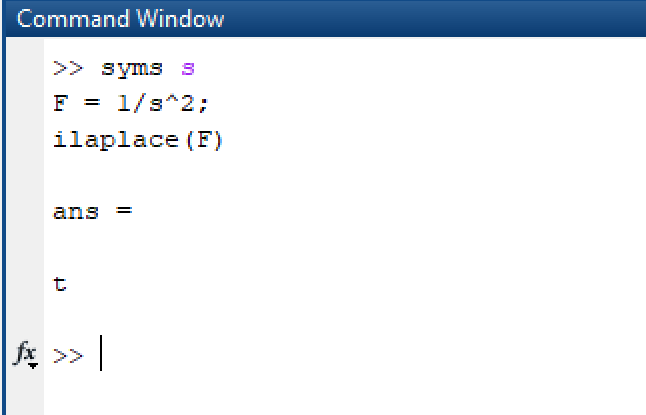
\includegraphics[width=0.6\linewidth]{Figuras/Ch03/fig2.PNG}}
}

\frame{
\frametitle{Frações parciais}
\begin{block}{Introdução}
Para sistemas lineares cujo modelo obtido é uma \textbf{equação diferencial ordinária} com coeficientes constantes, a função $F(s)$ que queremos inverter é sempre uma fração
em que o \textbf{numerador} $N(s)$ e o \textbf{denominador} $D(s)$ são polinômios em $s$, excetuando o caso em que existem termos de defasamento $e^{-sa}$. Estes termos são facilmente resolvidos com a aplicação do teorema do deslocamento no tempo. Logo, temos:
$$F(s) \triangleq \dfrac{N(s)}{D(s)}$$
em que:
\begin{itemize}
    \item $N(s) \triangleq$ polinômio em $s$ correspondente ao \textbf{numerador} de $F(s)$.
    \item $D(s) \triangleq$ polinômio em $s$ correspondente ao \textbf{denominador} de $F(s)$.
\end{itemize}
\end{block}
}

\frame{
\frametitle{Frações parciais}
\begin{block}{Procedimentos}
\begin{enumerate}
    \item Se o coeficiente de maior ordem de $D(s)$ não for igual à unidade, transforme-o.
    \item Se $N(s)$ tiver grau maior ou igual que $D(s)$, divida $N(s)$ por $D(s)$ para obter uma fração própria somada de outros termos.
    \item Fatore $D(s)$ usando as raízes do denominador, que poderão ser reais e/ou
    complexas.
    \item Faça a expansão em frações parciais.
    \item Após obter $F(s)$ em frações parciais, procure a correspondente função do tempo
    para cada fração e possíveis outros termos (do passo 2).
\end{enumerate}
\end{block}
}

\frame{
\frametitle{Frações parciais - Exemplo $\#01$}
\begin{block}{Problema}
$$F(s) = \dfrac{4s^4 + 32s^3 + 98s^2 + 116s + 38}{2s^3 + 12s^2 + 22s + 12}$$
\end{block}
}

\frame{
\frametitle{Frações parciais - Exemplo $\#01$}
\begin{block}{Resolução}
\begin{itemize}
    \item O primeiro passo é transformar o coeficiente que acompanha o termo $s^3$ no denominador igual à unidade.
\end{itemize}
$$F(s) = \dfrac{2s^4 + 16s^3 + 49s^2 + 58s + 19}{s^3 + 6s^2 + 11s + 6}$$
\begin{itemize}
    \item Como o grau do numerador é superior ao do denominador, devemos fazer divisões sucessivas. Após este procedimento, obtemos:
\end{itemize}
$$F(s) = 2s + 4 + \dfrac{3s^2 + 2s -5}{s^3 + 6s^2 + 11s + 6}$$
\end{block}
}

\frame{
\frametitle{Frações parciais - Exemplo $\#01$}
\begin{block}{Resolução}
\begin{itemize}
    \item Como a transformada inversa de Laplace é linear, temos:
\end{itemize}
$$\mathscr{L}^{-1}\{F(s)\} = \mathscr{L}^{-1}\{2s+4\} + \mathscr{L}^{-1}\ \Big\{\dfrac{3s^2 + 2s -5}{s^3 + 6s^2 + 11s + 6}\ \Big\}$$
\begin{itemize}
    \item Para o segundo termo da direita devemos fator as raízes do polinômio $D(s)$:
\end{itemize}
$$\mathscr{L}^{-1}\ \Big\{\dfrac{3s^2 + 2s -5}{s^3 + 6s^2 + 11s + 6}\ \Big\} =  \mathscr{L}^{-1}\ \Big\{\dfrac{3s^2 + 2s -5}{(s+1)(s+2)(s+3)}\ \Big\}$$
\end{block}
}

\cprotect\frame{
\frametitle{Frações parciais - Exemplo $\#01$}
\begin{block}{}
\begin{verbatim}
>>r=roots(p)
\end{verbatim}
retorna as raízes do polinômio representado por $\bm{p}$ como um vetor de coluna. A entrada $\bm{p}$ é um vetor contendo os $\bm{n+1}$ coeficientes polinomiais, começando com o coeficiente de $\bm{x^n}$ \\
\vspace{0.2cm}
\textbf{Exemplo}: calcule as raízes de $s^3 + 6s^2 + 11s + 6$
\end{block}
\centerline{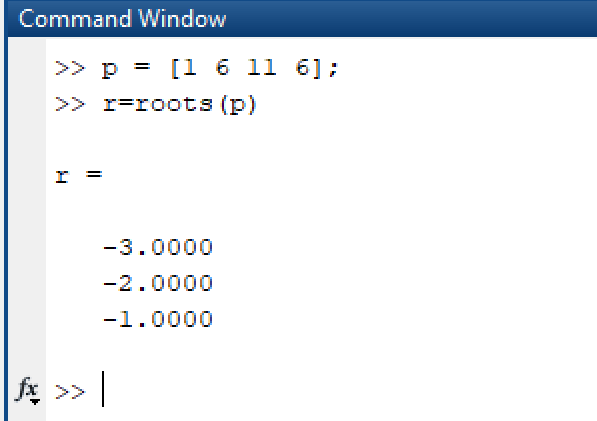
\includegraphics[width=0.5\linewidth]{Figuras/Ch03/fig3.PNG}}
}

\frame{
\frametitle{Frações parciais - Exemplo $\#01$}
\begin{block}{Resolução}
\begin{itemize}
    \item O próximo passo é a realização da expansão por frações parciais.
\end{itemize}
$$\dfrac{3s^2 + 2s -5}{s^3 + 6s^2 + 11s + 6} = \dfrac{A}{s+1} + \dfrac{B}{s+2} + \dfrac{C}{s+3}$$
$$A = F(s)(s+1)\Big|_{s=-1} = \dfrac{3s^2 + 2s -5}{(s+2)(s+3)}\Big|_{s=-1} = -2$$
$$B = F(s)(s+2)\Big|_{s=-2} = \dfrac{3s^2 + 2s -5}{(s+1)(s+3)}\Big|_{s=-2} = -3$$
$$C = F(s)(s+3)\Big|_{s=-3} = \dfrac{3s^2 + 2s -5}{(s+1)(s+2)}\Big|_{s=-3} = 8$$
\end{block}
}

\cprotect\frame{
\frametitle{Frações parciais - Exemplo $\#01$}
\begin{block}{}
\begin{verbatim}
>>[r,p,k] = residue(n,d)
\end{verbatim}
encontra os coeficientes ($\bm{r}$), os polos ($\bm{p}$) e os termos diretos ($\bm{k}$) de uma expansão em frações parciais.
\end{block}
\centerline{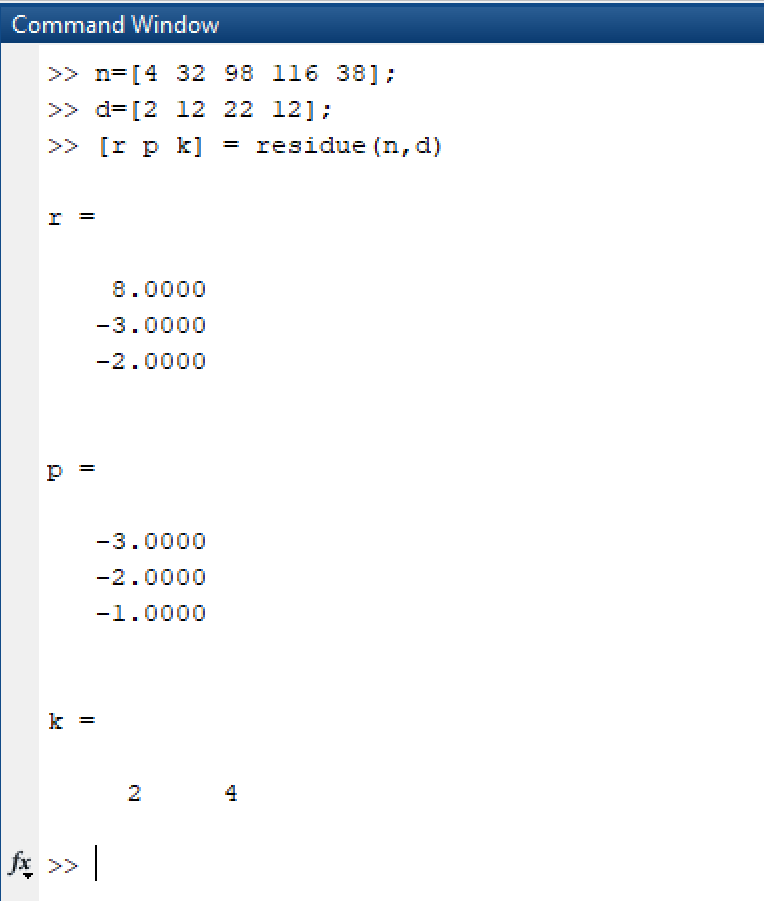
\includegraphics[width=0.4\linewidth]{Figuras/Ch03/fig4.PNG}}
}

\frame{
\frametitle{Frações parciais - Exemplo $\#01$}
\begin{block}{Resolução}
\begin{itemize}
    \item Deste modo, a transformada inversa de Laplace da segunda parte é dada por:
\end{itemize}
$$\mathscr{L}^{-1}\ \Big\{\dfrac{3s^2 + 2s -5}{s^3 + 6s^2 + 11s + 6}\ \Big\} =  \mathscr{L}^{-1}\ \Big\{\dfrac{-2}{s+1} + \dfrac{-3}{s+2} + \dfrac{8}{s+3}\ \Big\}$$
$$= -2e^{-t}-3e^{-2t}+8e^{-3t}$$
\begin{itemize}
    \item A transformada inversa de Laplace da primeira parte parte é dada por:
\end{itemize}
$$\mathscr{L}^{-1}\{2s+4\} = 2 \ \mathscr{L}^{-1}\{s\} + 4 \ \mathscr{L}^{-1}\{1\} = 2\dot{\delta}(t) + 4\delta(t) $$
\begin{itemize}
    \item A resposta final é, portanto:
\end{itemize}
$$\boxed{f(t) = 2\dot{\delta}(t) + 4\delta(t) -2e^{-t}-3e^{-2t}+8e^{-3t}}$$
\end{block}
}

\frame{
\frametitle{Frações parciais - Exemplo $\#02$}
\begin{block}{Problema}
$$F(s) = \dfrac{18s^2 + 36s + 24}{(6s+6)(s+2)^3}$$
\end{block}
}

\frame{
\frametitle{Frações parciais - Exemplo $\#02$}
\begin{block}{Resolução}
\begin{itemize}
    \item O primeiro passo é transformar o coeficiente que acompanha o termo $s^4$ no denominador igual à unidade.
\end{itemize}
$$F(s) = \dfrac{3s^2 + 6s + 4}{(s+1)(s+2)^3}$$
\end{block}
}

\frame{
\frametitle{Frações parciais - Exemplo $\#02$}
\begin{block}{Resolução}
\begin{itemize}
    \item O próximo passo é a realização da expansão por frações parciais. Perceba que neste caso temos raízes com multiplicidade.
\end{itemize}
$$\dfrac{3s^2 + 6s +4}{(s+1)(s+2)^3} = \dfrac{A}{s+1} + \dfrac{B_3}{(s+2)^3} + \dfrac{B_2}{(s+2)^2} + \dfrac{B_1}{s+2}$$
$$A = F(s)(s+1)\Big|_{s=-1} = \dfrac{3s^2 + 6s +4}{(s+2)^3}\Big|_{s=-1} = 1$$
$$B_3 = F(s)(s+2)^3\Big|_{s=-2} = \dfrac{3s^2 + 6s + 4}{(s+1)}\Big|_{s=-2} = -4$$
\end{block}
}

\frame{
\frametitle{Frações parciais - Exemplo $\#02$}
\begin{block}{Resolução}
\begin{itemize}
    \item Por sua vez, os coeficientes $B_2$ e $B_1$ devem ser calculados através de outro
    procedimento, que é a equação dada abaixo.
\end{itemize}
$$B_n = \Big\{\dfrac{1}{(m-n)!}  \dfrac{\text{d}^{m-n}}{\text{d}s^{m-n}} \big[(s-s_1)^m F(s)\big] \Big\}\Big|_{s=s_1}$$
em que:
\begin{itemize}
    \item $m \triangleq$ número de vezes que o polo $s_1$ aparece
    \item $n \triangleq$ índice do numerador da fração parcial
\end{itemize}
\vspace{0.3cm}
$$B_2 = \Big\{\dfrac{1}{1!}  \dfrac{\text{d}}{\text{d}s} \big[(s+2)^3 F(s)\big] \Big\}\Big|_{s=-2} = 2$$
$$B_1 = \Big\{\dfrac{1}{2!}  \dfrac{\text{d}^2}{\text{d}s^2} \big[(s+2)^3 F(s)\big] \Big\}\Big|_{s=-2} = 1$$
\end{block}
}

\frame{
\frametitle{Frações parciais - Exemplo $\#02$}
\begin{block}{Resolução}
\begin{itemize}
    \item Deste modo, a transformada inversa de Laplace é dada por:
\end{itemize}
$$\mathscr{L}^{-1}\ \Big\{\dfrac{3s^2 + 6s +4}{(s+1)(s+2)^3}\ \Big\} =  \mathscr{L}^{-1}\ \Big\{\dfrac{1}{s+1} + \dfrac{-4}{(s+2)^3} + \dfrac{2}{(s+2)^2} + \dfrac{1}{s+2} \ \Big\}$$
$$= e^{-t}-2t^2e^{-2t}+2te^{-2t}+e^{-2t}$$
\begin{itemize}
    \item A resposta final é, portanto:
\end{itemize}
$$\boxed{f(t) = e^{-t}-2t^2e^{-2t}+2te^{-2t}+e^{-2t}}$$
\end{block}
}

\frame{
\frametitle{Frações parciais - Exemplo $\#03$}
\begin{block}{Problema}
$$F(s) = \dfrac{3s+1}{s^3-s^2+s-1}$$
\end{block}
}

\frame{
\frametitle{Frações parciais - Exemplo $\#03$}
\begin{block}{Resolução}
\begin{itemize}
    \item Em primeiro lugar devemos encontrar as raízes do polinômio $D(s)$, fatorando-o.
\end{itemize}
$$F(s) = \dfrac{3s+1}{(s-1)(s^2+1)}$$
\end{block}
}

\frame{
\frametitle{Frações parciais - Exemplo $\#03$}
\begin{block}{Resolução}
\begin{itemize}
    \item O próximo passo é a realização da expansão por frações parciais. Perceba que neste caso temos raízes complexas conjugadas.
\end{itemize}
$$\dfrac{3s+1}{(s-1)(s^2+1)} = \dfrac{A}{s-1} + \dfrac{Bs+C}{s^2+1} = \dfrac{A}{s-1} + \dfrac{Bs}{s^2+1} + \dfrac{C}{s^2+1}$$
\begin{itemize}
    \item Um método alternativo é a resolução por comparação de polinômios:
\end{itemize}
\begin{align*}
    3s+1 &= A(s^2+1) + Bs(s-1) + C(s-1) \\
    3s + 1 &= (A+B)s^2 + (-B+C)s + A-C
\end{align*}
\begin{equation*}
\begin{cases}
A + B = 0 \\
-B + C = 3 \\
A - C = 1
\end{cases}
\end{equation*}
\vspace{-0.2cm}
\begin{itemize}
    \item Daí, $A = 2$, $B = -2$ e $C = 1$
\end{itemize}
\end{block}
}

\frame{
\frametitle{Frações parciais - Exemplo $\#03$}
\begin{block}{Resolução}
\begin{itemize}
    \item Deste modo, a transformada inversa de Laplace é dada por:
\end{itemize}
$$\mathscr{L}^{-1}\ \Big\{\dfrac{3s+1}{(s-1)(s^2+1)}\ \Big\} =  \mathscr{L}^{-1}\ \Big\{\dfrac{2}{s-1} + \dfrac{-2s}{s^2+1} + \dfrac{1}{s^2+1} \ \Big\}$$
$$= 2e^{t}-2\text{cos}(t)+\text{sen}(t)$$
\begin{itemize}
    \item A resposta final é, portanto:
\end{itemize}
$$\boxed{f(t) = 2e^{t}-2\text{cos}(t)+\text{sen}(t)}$$
\end{block}
}

\frame{
\frametitle{Frações parciais - Exemplo $\#04$}
\begin{block}{Problema}
$$F(s) = \dfrac{100(s+3)}{(s+6)(s^2+6s+25)}$$
\end{block}
}

\frame{
\frametitle{Frações parciais - Exemplo $\#04$}
\begin{block}{Resolução}
\begin{itemize}
    \item Em primeiro lugar devemos encontrar as raízes do polinômio $D(s)$, fatorando-o.
\end{itemize}
$$F(s) = \dfrac{100(s+3)}{(s+6)(s+3-j4)(s+3+j4)}$$
\end{block}
}

\frame{
\frametitle{Frações parciais - Exemplo $\#04$}
\begin{block}{Resolução}
\begin{itemize}
    \item O próximo passo é a realização da expansão por frações parciais. Perceba que neste caso temos raízes complexas conjugadas.
\end{itemize}
$$\dfrac{100(s+3)}{(s+6)(s+3-j4)(s+3+j4)} = \dfrac{A}{s+6} + \dfrac{B}{s+3-j4} + \dfrac{C}{s+3+j4}$$
\begin{itemize}
    \item O próximo passo é a realização da expansão por frações parciais.
\end{itemize}
$$A = F(s)(s+6)\Big|_{s=-6} = \dfrac{100(s+3)}{s^2+6s+25}\Big|_{s=-6} = -12$$
$$B = F(s)(s+3-j4)\Big|_{s=-3+j4} = \dfrac{100(s+3)}{(s+6)(s+3+j4)}\Big|_{s=-3+j4} =$$ 
$$= \dfrac{j400}{(3+j4)j8} = \dfrac{50}{3+j4} = 6 - j8$$
\begin{itemize}
    \item De acordo com o Teorema das raízes complexas, $C = 6 + j8$
\end{itemize}
\end{block}
}

\frame{
\frametitle{Frações parciais - Exemplo $\#04$}
\begin{block}{Resolução}
\begin{itemize}
    \item Deste modo, a transformada inversa de Laplace é dada por:
\end{itemize}
$$\mathscr{L}^{-1}\ \Big\{\dfrac{100(s+3)}{(s+6)(s^2+6s+25)}\ \Big\} =  \mathscr{L}^{-1}\ \Big\{\dfrac{-12}{s+6} + \dfrac{6-j8}{s+3-j4} + \dfrac{6+j8}{s+3+j4} \ \Big\}$$
$$= -12e^{-6t} + (6-j8)e^{-(3-j4)t} + (6+j8)e^{-(3+j4)t}$$
\begin{itemize}
    \item Expandindo o segundo termo na fórmula de Euler, temos:
\end{itemize}
$$(6-j8)e^{-(3-j4)t} = (6-j8) \ e^{j4t} \ e^{-3t} = (6-j8) \ [\text{cos}(4t) + j\text{sen}(4t)] \ e^{-3t}$$ 
$$= \big(6\text{cos}(4t) +j6\text{sen}(4t) - j8\text{cos}(4t) + 8\text{sen}(4t)\big) \ e^{-3t}$$

\begin{itemize}
    \item Expandindo o terceiro termo na fórmula de Euler, temos:
\end{itemize}
$$(6+j8)e^{-(3+j4)t} = (6+j8) \ e^{-j4t} \ e^{-3t} = (6+j8) \ [\text{cos}(4t) - j\text{sen}(4t)] \ e^{-3t}$$ 
$$= \big(6\text{cos}(4t) -j6\text{sen}(4t) +j8\text{cos}(4t) + 8\text{sen}(4t)\big) \ e^{-3t}$$
\end{block}
}

\frame{
\frametitle{Frações parciais - Exemplo $\#04$}
\begin{block}{Resolução}
\begin{itemize}
    \item Deste modo, a transformada inversa de Laplace é dada por:
\end{itemize}
$$\mathscr{L}^{-1}\ \Big\{\dfrac{100(s+3)}{(s+6)(s^2+6s+25)}\ \Big\} =  \mathscr{L}^{-1}\ \Big\{\dfrac{-12}{s+6} + \dfrac{6-8i}{s+3-4i} + \dfrac{6+8i}{s+3+4i} \ \Big\}$$
$$= -12e^{-6t} + 12e^{-3t}\text{cos}(4t) + 16e^{-3t}\text{sen}(4t)$$
\begin{itemize}
    \item A resposta final é, portanto:
\end{itemize}
$$\boxed{f(t) = -12e^{-6t} + 12e^{-3t}\text{cos}(4t) + 16e^{-3t}\text{sen}(4t)}$$
\end{block}
}

\frame{
\frametitle{Exercícios}
\begin{block}{}
01. Sabendo que $F(s) = \dfrac{3s+7}{s^2-2s-3}$, determine $f(t)$.

\vspace{1cm}

02. Determine $g(t)$ dado que $G(s) = \dfrac{5s^2-15s-11}{s^4-5s^3+6s^2+4s-8}$.
\end{block}
}

\frame{
\frametitle{Referências e exercícios complementares}
\begin{itemize}
\item HAYKIN, Simon S.; VEEN, Barry B. Signals and Systems, 2 ed. John Wiley \& Sons, 2005.
\end{itemize}
\centering{\alert{Página 546 - \textbf{Capítulo 6}}} \\
}